\chapter{Produktidee}

\section{Einleitung}

Das effektive und vor allem zeit- und energieoptimale Ansteuern von Roboterarmen stellt trotz modernster Rechner, wegen der hohen Problemkomplexität, eine große Herausforderung dar. Es ist bis heute nicht gelungen einen Algorithmus zu entwerfen der dieses Problem optimal löst und daher arbeiten alle Anlagen mit Näherungslösungen für die optimale Pfadplanung.

Unsere Idee ist es ein künstliches Neuronales Netzwerk auf die Lösung dieses Problems zu trainieren, umso eine höhere Energieeffizienz und Geschwindigkeit des Roboterarmes zu erreichen.
Dieses Konzept ist inspiriert vom Menschen selbst. Jede Bewegung die man ausführt wird vom Gehirn automatisch darauf optimiert wird mit möglichst geringem Aufwand durgeführt zu werden und das ohne davor eine komplette Planung der Bewegung zu benötigen. Wir wollen dieses Konzept auf Industrieroboter übertragen und so das Problem der Trajektorienplanung lösen.

\section{Umsetzung}

Zur Umsetzung einer Robotersteuerung gibt es grundsätzlich zwei Ansätze. Bei dem ersten Ansatz wird vor dem Losfahren offline eine Trajektorie berechnet, welche anschließend als Liste von Punkten zum Roboter übertragen werden.  Diese werden nacheinander linear angefahren. Der zweite Ansatz ist das Online-planing, hierbei entfällt die Wartezeit vor dem Verfahren und der Roboter versucht sofort, anhand eines Algorithmus, seine Zielposition zu erreichen. 

Die Vorteile unseres Ansatzes mit einem Neuronalen Netzwerk (NN) liegen darin, dass die Modellbildung durch ein Neuronales Netzwerk sämtliche physikalischen Effekte in der Mechanik des Roboters, wie Nichtlineare-Reibungen berücksichtigt, was mit etablierten Ansätzen nur teilweise möglich ist.

Vorangegangene Prototypen für eine NN basierte Regelung der Roboterarmgelenke haben gezeigt, dass Effizienzsteigerungen von bis zu 50\% im Vergleich zu herkömmlichen Algorithmen möglich sind. Die so erzeugten Trajektorien sind nicht nur Energiesparender, sondern auch schonender für die Mechanik, da sie sanftere Beschleunigungs- und Bremsvorgänge einzelner Gelenke verwenden. Durch die optimierte Trajektorie wird die Gesamtzeit zum Erreichen des Zielpunktes jedoch nicht verlängert, sondern kann in vielen Fällen sogar reduziert werden.

\begin{figure}[h]
	\centering
	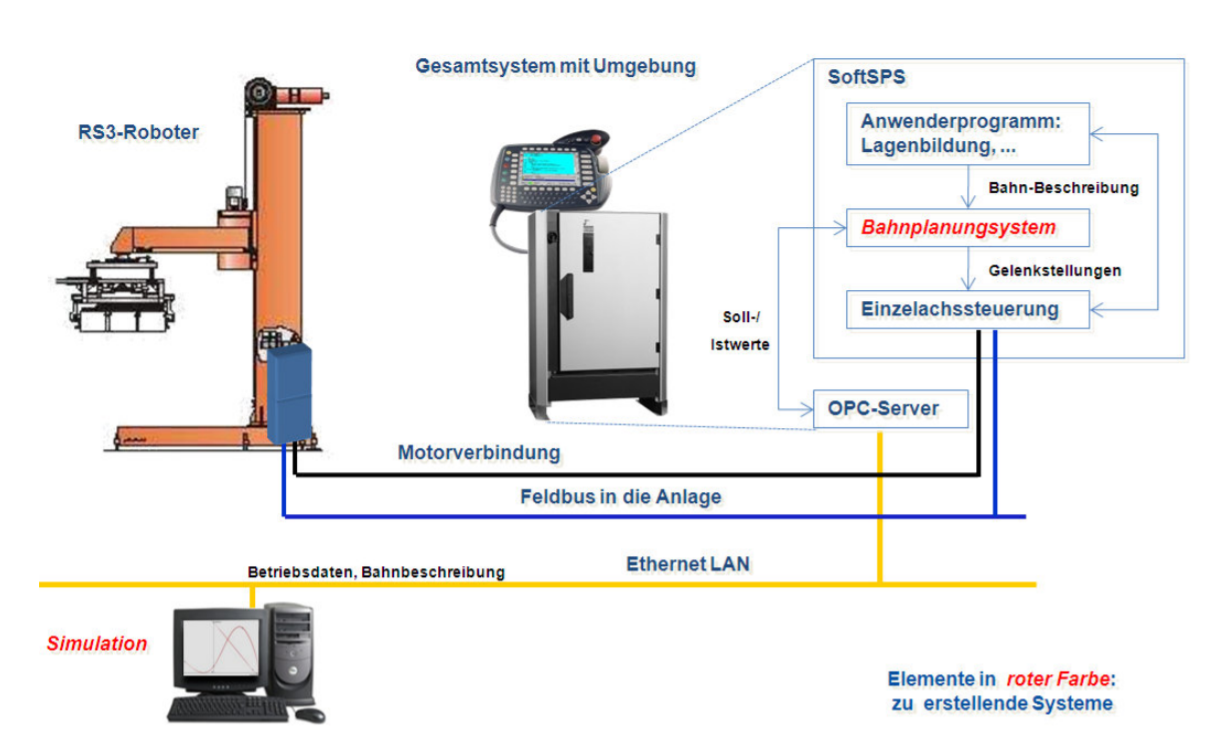
\includegraphics[width=15cm]{sytem_overview.png}
	\caption{Integrierung eines neuen Bahnplanungssystems in eine bestehende Roboterzelle}
	\label{fig:IntegrationBahnplanungssystem}
\end{figure}

Unser Produkt ist ausschließlich die Software, welche auf der Robotersteuerung läuft und die Regelung übernimmt und umfasst keine Hardware. Auf diese Weise wollen wir uns voll auf unsere Hauptkompetenz fokussieren. 
